
\chapter{Introducción al Lenguaje C}


El lenguaje de programación C fue creado en 1972 por investigadores de 
Bell Telephone Laboratories, con el objetivo de reescribir un sistema
operativo, el UNIX, en un lenguaje de alto nivel, para poder adaptarlo
(es decir, \textit{portarlo}) a diferentes arquitecturas. Por este motivo sus
creadores se propusieron metas de diseño especiales, tales como: 

\begin{itemize}
\item Poder utilizar todos los recursos del hardware (\quotes{acceso al bajo nivel}). 
\item Obtener código generado eficiente en uso de memoria y en tiempo de ejecución (programas pequeños y veloces).
\item Compilador portable (implementable en cualquier arquitectura).
\end{itemize}


Actualmente existen implementaciones de C para todas las arquitecturas y
sistemas operativos, y es el lenguaje más utilizado para la
\textbf{programación de sistemas}. Por su gran eficiencia resulta ideal para
la programación de \textbf{sistemas operativos}, \textbf{drivers de dispositivos},
\textbf{herramientas de programación}. El 95\% del sistema operativo UNIX
está escrito en C, así como gran parte de los modernos
sistemas y ambientes operativos, y los programas de administración o aplicación que corren
sobre ellos.

%TODO
%\href{info/info1.html#info1}{Mas información ...} 

\section{Características del lenguaje}
C es un lenguaje compilado. Sintácticamente, presenta similitudes formales 
con C++, con Java, y aun con Pascal, pero las diferencias en otros aspectos son muy
importantes. A pesar de permitir \textbf{operaciones de bajo nivel}, tiene las
\textbf{estructuras de control}, y permite la \textbf{estructuración de datos}, propias
de los lenguajes procedurales de alto nivel. 

\subsection{Paradigma procedural}
El lenguaje C \textbf{no es un lenguaje orientado a objetos}, sino que
adhiere al paradigma tradicional de \textbf{programación imperativa o procedural}. No
soporta la orientación a objetos propiamente dicha, al no
proporcionar herramientas fundamentales, como la herencia. Sin embargo,
algunas características del lenguaje permiten que un proyecto de
programación se beneficie, de todas maneras, con la aplicación de
algunos principios de la orientación a objetos, tales como el
ocultamiento de información y el encapsulamiento de
responsabilidades. El lenguaje \textbf{C++}, orientado a objetos, \textbf{no es}
una versión más avanzada del lenguaje o un compilador de C con
más capacidades, sino que \textbf{se trata de un lenguaje completamente
diferente}. 


\subsection{Minimalidad}
Un programa en C es, por lo general, más \textbf{sintético} que en otros
lenguajes procedurales; la idea central que atraviesa todo
el lenguaje es la minimalidad. La definición del lenguaje consta de
muy pocos elementos, y tiene muy pocas \textbf{palabras reservadas}. 

Como rasgo distintivo, en C no existen, rigurosamente hablando, funciones o
procedimientos de uso general del programador. Por ejemplo, \textbf{no tiene
funciones de entrada/salida}; la definición del lenguaje apenas
alcanza a \textbf{las estructuras de control y los operadores}. La idea de
definir un lenguaje sin funciones es, por un lado, hacer posible que el
compilador sea \textbf{pequeño, fácil de escribir e inmediatamente
portable}; y por otro, permitir que sea el usuario quien defina sus
propias funciones cuando el problema de programación a resolver tenga
requerimientos especiales. El usuario puede escribir sus propios procedimientos (llamados
\textbf{funciones} aunque no devuelvan valores). Aunque existe la
noción de \textbf{bloque} de sentencias (sentencias encerradas entre llaves), el lenguaje se dice \textbf{\textit{no}
estructurado en bloques} porque no pueden definirse funciones dentro de
otras. 

\subsection{Versatilidad, a un precio}
El lenguaje entrega completamente el control de la máquina subyacente
al programador, no realizando controles en tiempo de ejecución. Es
decir, no verifica condiciones de error comunes como \textbf{\textit{overflow}
de variables}, \textbf{errores de entrada/salida}, o \textbf{consistencia de argumentos}
en llamadas a funciones. Ofrece una gran libertad sintáctica al programador. No
es fuertemente tipado. Cuando es necesario, se realizan \textbf{conversiones
automáticas de tipo} en las asignaciones, a veces \textbf{con efectos
laterales inconvenientes} si no se tiene precaución. Una función que
recibe determinados parámetros formales puede ser invocada con
argumentos reales de otro tipo. 

Se ha dicho que estas características
\quotes{liberales} posibilitan la realización de
proyectos complejos con más facilidad que otros lenguajes como Pascal
o Ada, más estrictos; aunque al mismo tiempo, así resulta más
difícil detectar errores de programación en tiempo de
compilación. Como resultado, es frecuente que el
principiante, y aun el experto, cometan errores de programación que
no se hacen evidentes enseguida, ocasionando problemas y costos de
desarrollo. En este sentido, según los partidarios de la
tipificación estricta, C no es un buen lenguaje. Gran parte del
esfuerzo de desarrollo del estándar ANSI se dedicó a dotar al C de
elementos para mejorar esta deficiencia. 

Una característica especial del lenguaje C es que el \textbf{pasaje de
argumentos a funciones} se realiza siempre \textbf{por valor}. ¿Qué ocurre
cuando una función debe \textbf{modificar} datos que recibe como
argumentos? La única salida es pasarle --por valor-- la dirección del
dato a modificar. Las consecuencias de este hecho son más fuertes de
lo que parece a primera vista, ya que surge la necesidad de todo un
conjunto de técnicas de \textbf{manejo de punteros} que no siempre son bien
comprendidas por los programadores poco experimentados, y abre la
puerta a sutiles y escurridizos errores de programación. Quizás
este punto, junto con el de la ausencia de comprobaciones en tiempo de
ejecución, sean los que le dan al C fama de \quotes{difícil
de aprender}. 

\subsection{Portabilidad}
Los \textbf{tipos de datos} no tienen un tamaño determinado por la definición
del lenguaje, sino que diferentes implementaciones pueden adoptar
diferentes convenciones. Paradójicamente, esta característica
obedece al objetivo de lograr la \textbf{portabilidad} de los programas en C. El
programador está obligado a no hacer ninguna suposición sobre los
tamaños de los \textbf{objetos de datos}, ya que lo contrario haría al
software dependiente de una arquitectura determinada (\quotes{no portable}). 



\subsection{Biblioteca Standard}
Pese a no estar formalmente definidas funciones de entrada/salida en el lenguaje, se ha establecido un conjunto mínimo de funciones,
llamado la \textbf{Biblioteca Standard} del lenguaje C, que todos los
compiladores proveen, a veces con agregados. La filosofía de la
Biblioteca Standard es la portabilidad, es decir, casi no incluye
funciones que sean específicas de un sistema operativo determinado.
Aquellas que sí incluye están orientadas a la programación de sistemas, y a
veces no resultan suficientes para el programador de aplicaciones. No
provee, por ejemplo, la capacidad de manejo de archivos indexados, ni
funciones de entrada/salida interactiva por consola que sean seguras
(\quotes{a prueba de usuarios}). Estas deficiencias
se remedian utilizando bibliotecas de funciones \quotes{de
terceras partes} (creadas por el usuario u obtenidas de
otros programadores). 

Las funciones de la Biblioteca Standard no tienen ningún
privilegio sobre las del usuario y \textbf{sus nombres no son palabras
reservadas}; el usuario puede reemplazarlas por sus propias funciones
simplemente dándoles el mismo nombre. 


\section{Evolución del lenguaje}
La primera definición oficial del lenguaje fue dada en 1978 por
\textbf{Brian Kernighan y Dennis Ritchie} (Fig. \ref{fig:kandr}) en su libro \textbf{El
lenguaje de programación C}. Este lenguaje fue llamado
\textbf{C K\&R}, por las iniciales de sus autores. En 1983 se creó el comité
ANSI para el lenguaje, que en 1988 estableció el estándar ANSI C, con algunas reformas
sobre el C K\&R. Simultáneamente, Kernighan y Ritchie publicaron la
segunda edición de su libro, describiendo la mayor parte de las
características del ANSI C. 


 \begin{figure}[htbp] 
 \centering 
 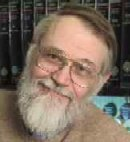
\includegraphics[width=3.44cm,height=3.969cm]{./img/kernighan.jpg} 
 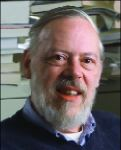
\includegraphics[width=3.44cm,height=3.969cm]{./img/dennis_ritchie.jpg} 
 \caption{Brian Kernighan y Dennis Ritchie, los creadores del lenguaje C} 
 \label{fig:kandr} 
 \end{figure} 


Algunas nuevas características de C99 son: 

\begin{itemize}
\item Matrices de tamaño variable 
\item Soporte de números complejos 
\item Tipos \code{long long int} y \code{unsigned long long int} de al menos 64 bits 
\item Familia de funciones \code{vscanf()} 
\item Comentarios al estilo de C++ prefijando las líneas con la secuencia \code{//}. 
\item Familia de funciones \code{snprintf()} 
\item Tipo boolean
\end{itemize}

%TODO C11

\section{El ciclo de compilación}
Las herramientas esenciales de un ambiente de desarrollo, además de
cualquier \textbf{editor de textos}, son el \textbf{compilador}, el \textbf{vinculador}, 
\textbf{linkeditor} o \textit{linker}, y el \textbf{bibliotecario}. A
estas herramientas básicas se agregan otras, útiles para
automatizar la compilación de proyectos extensos, almacenar y
recuperar versiones de programas fuente, comprobar sintaxis en forma
previa a la compilación, etc. Según el ambiente operativo y
producto de software de que se trate, estas herramientas pueden ser comandos de línea independientes, con
salidas de texto simples, o encontrarse integradas en una interfaz de usuario uniforme, en modo
texto o modo gráfico. 

Cuando encontramos varias de estas herramientas integradas en una sola aplicación, decimos que se trata de un \textbf{IDE} (\textit{Integrated Development Environment}) o ambiente de desarrollo integrado. Un IDE oculta el ciclo de compilación al usuario, con la intención de simplificar el proceso de desarrollo. Sin embargo, conviene conocer qué función se cumple, y qué producto se espera, en cada fase del ciclo de compilación, para poder interpretar las diferentes situaciones de error y poder corregirlas.

\figura[12]{ciclo}{El ciclo de compilación produce un ejecutable a partir de archivos fuente.}{ciclo.eps}

\subsection{Compilador}
\begin{itemize}
	\item El compilador acepta un archivo \textbf{fuente}, posiblemente relacionado con
otros (una \textbf{unidad de traducción}), y genera con él un
\textbf{módulo objeto}. Este módulo objeto contiene porciones de
código ejecutable mezclado con \textbf{referencias}, aún no resueltas, a
variables o funciones cuya definición no figura en los fuentes de
entrada. Estas referencias quedan en forma simbólica en el módulo
objeto hasta que se resuelvan en un paso posterior. 
\item Si ocurren errores en esta fase, se deberán a problemas de sintaxis (el código escrito por el programador no respeta la definición del lenguaje).
\end{itemize}

\subsection{Vinculador, linkeditor o \textit{linker}}
\begin{itemize}
\item El vinculador recibe como entrada un conjunto de módulos objeto y
busca \textbf{resolver}, vincular, o enlazar, las referencias simbólicas en ellos,
buscando la definición de las variables o funciones faltantes en los
mismos objetos o en bibliotecas. Éstas pueden ser la Biblioteca
Standard, u otras provistas por el usuario. Cuando el linker encuentra la
definición de un objeto buscado (es decir, de una variable o
función), la copia en el archivo resultante de salida (la
\textit{resuelve}). El objetivo del linker es resolver todas las
referencias pendientes para producir un programa ejecutable. 
\item Si ocurren errores en esta fase, se deberán a que existen variables o funciones cuya definición no ha sido dada (no se encuentran en las unidades de traducción procesadas, ni en ninguna biblioteca conocida por el linker).
\end{itemize}

\subsection{Bibliotecario}
\begin{itemize}
	\item El bibliotecario es un programa administrador de módulos objeto. Su función
es reunir módulos objeto en archivos llamados \textbf{bibliotecas}, y luego
permitir la extracción, borrado, reemplazo y agregado de módulos.
El conjunto de módulos en una biblioteca se completa con una tabla de
información sobre sus contenidos para que el linker pueda encontrar
rápidamente aquellos módulos donde se ha definido una variable o
función, y así extraerlos durante el proceso de linkedición. 
\item El bibliotecario es utilizado por el usuario cuando desea mantener sus
propias bibliotecas. La creación de bibliotecas propias del usuario
ahorra tiempo de compilación y permite la distribución de software
sin revelar la forma en que se han escrito los fuentes y
protegiéndolo de modificaciones. 
\end{itemize}

Una vez que el código ha sido compilado y vinculado, obtenemos un programa ejecutable. Los errores que pueden producirse en la ejecución ya no corresponden a problemas de compilación, sino que se deben a aspectos de diseño del programa que deben ser corregidos por el programador.

\section{Un primer ejemplo}

El clásico ejemplo de todas las introducciones al lenguaje C es un programa llamado \quotes{\textbf{Hello, World!}}.

\begin{lstlisting}
#include <stdio.h>
/* El primer programa! */
main()
{
	printf("Hola, gente!\n");
}
\end{lstlisting}

\subsection{Estructura del programa}

\begin{itemize}
\item Este programa minimal comienza con una \textbf{directiva de preprocesador} que indica incluir en la unidad de traducción al
archivo de cabecera o \textit{header} \textbf{stdio.h}. Éste contiene, entre otras
cosas, la declaración (o \textbf{prototipo}) de la función de
salida de caracteres \textbf{printf()}, perteneciente a la Biblioteca Standard. Los prototipos se incluyen para
advertir al compilador de los tipos de las funciones y de sus
argumentos. 
\item Entre los pares de caracteres especiales \textbf{/*} y \textbf{*/}se puede insertar cualquier cantidad de líneas de comentarios. 
\item La función \textbf{main()} es el cuerpo principal del programa
(es por donde comenzará la ejecución). Todas las funciones en C están delimitadas por un par de llaves. Terminada la ejecución de
main(), terminará el programa. 
\item La función \code{printf()} imprimirá la cadena entre comillas, que es
una \textbf{constante string} terminada por un carácter de
\textbf{nueva línea} (la secuencia especial \quotes{\code{\\n}}). 
\end{itemize}

\subsection{Compilación del programa}
Para ver el primer ejemplo en C en funcionamiento:

\begin{enumerate}
	\item Copiar el programa con cualquier editor de textos y guardarlo en un archivo llamado \code{hola.c} en el directorio de trabajo del usuario.
	\item Sin cambiar de directorio, invocar al compilador ejecutando el comando \code{gcc hola.c -o hola}. Por defecto, el compilador \textbf{gcc} invocará al vinculador \textbf{ld} para generar el ejecutable a partir del archivo objeto intermedio generado. 
	\item Ejecutar el programa con el comando \code{./hola}. 
\end{enumerate}

Notar el \textit{punto y barra} del principio al ejecutar el programa. El punto y barra le indican al \textbf{shell} que debe buscar el programa en el directorio activo.

\subsubsection{Otra manera} 
%Lo mismo, pero de otra manera:
\begin{enumerate}
	\item Como antes, copiar el programa, o usar el mismo archivo fuente de hace un momento.
	\item Sin cambiar de directorio, ejecutar el comando \code{make hola} en una consola o terminal.
	\item Ejecutar el programa con el comando \code{./hola}. 
\end{enumerate}

La diferencia es que en el primer caso invocamos directamente al compilador \code{gcc},
mientras que en el segundo caso utilizamos la herramienta \code{make}, que nos asiste en la compilación de proyectos. En el ejemplo, le decimos al compilador que procese el archivo fuente \code{hola.c}, y que el ejecutable de salida (opción \code{-o}, de \textit{output}) reciba el nombre \code{hola}. 


% \subsection[Mapa de memoria de un programa Mas información ... ]{Mapa de memoria de un programa \href{info/info1.html#info2}{Mas información ...} }

\subsection{El comando make}
Cuando damos un comando como \code{make hola}, utilizamos el comando \textbf{make} para compilar y vincular el programa \textbf{hola.c}. El comando \textbf{make} contiene la inteligencia para:
\begin{itemize}
 	\item buscar, en el directorio activo, archivos fuente llamados \textbf{hola.*}; 
 	\item determinar (a partir de la extensión) que el hallado se trata de un programa en C;
 	\item ver que no existe en el directorio activo un programa ejecutable llamado \textbf{hola}, o que, si existe, su fecha de última modificación es anterior a la del fuente;
 	\item razonar que, por lo tanto, es necesario compilar el fuente \textbf{hola.c} para producir el ejecutable \textbf{hola};  
 	\item e invocar con una cantidad de opciones por defecto al compilador \textbf{gcc}, y renombrar la salida con el nombre
\textbf{hola}. Éste será el ejecutable que deseamos producir.
\end{itemize} 

Si se invoca al comando \textbf{make} una segunda vez, éste comprobará, en base a las fechas de
modificación de los archivos fuente y ejecutable, que no es necesaria la compilación (ya que el
ejecutable es posterior al fuente). Si editamos el fuente para cambiar algo en el programa, invocar
nuevamente a \textbf{make} ahora repetirá la compilación (porque ahora el fuente es posterior al ejecutable).

%TODO
%\subsection{Makefiles}


\section{Mapa de memoria de un programa}
Luego de la compilación y vinculación, el programa ejecutable queda contenido en un archivo. Al ser invocado, el sistema operativo lo carga en memoria, y allí se despliega en una cantidad de secciones de diferentes tamaños y con distintas funciones. 

Los sistemas operativos modernos, salvo raras excepciones, administran la memoria física  usando sistemas de memoria virtual. Cada sistema de memoria virtual funciona de modo diferente. La manera como se distribuyen realmente las secciones de un programa en la memoria física depende fuertemente de la
forma de administración de memoria del sistema operativo para el cual ha sido compilado y vinculado. Sin embargo,
el siguiente modelo puede servir de referencia para ilustrar algunas particularidades y problemas
que irán surgiendo con el estudio del lenguaje.

El programa cargado en memoria (Fig. \ref{fig:mapa}) se dividirá en cuatro regiones: código o \textbf{texto}, \textbf{datos
estáticos}, \textbf{heap} (o región de datos dinámicos), y \textbf{stack} (o pila). 

El tamaño de las regiones de código y de datos estáticos está determinado al momento de compilación
y es inamovible. Las otras dos regiones quedan en un bloque cuyo tamaño inicial es ajustado por el
sistema operativo al momento de la carga, pero puede variar durante la ejecución. Este bloque es
compartido entre ambas regiones. Una de ellas, la de datos dinámicos, o heap, crece \quotes{hacia arriba} (hacia 
direcciones de memoria más altas); la otra, la pila del programa, o stack, crece \quotes{hacia abajo} (en
sentido opuesto).


\figura[4]{mapa}{El mapa de memoria de un programa se divide conceptualmente en cuatro regiones}{mapadememoria.eps}

\begin{description}
	\item[Texto del programa] La región de texto contendrá el \textbf{código del programa}, es decir, la versión ejecutable de las
\textbf{instrucciones} que escribió el programador, traducidas por el compilador al lenguaje de la máquina. En
general, el programa fuente C se compondrá de funciones, que serán replicadas a nivel de máquina por
subrutinas en el lenguaje del procesador subyacente. Algunas instrucciones C resultarán en última
instancia en invocaciones a funciones del sistema (por ejemplo, cuando necesitamos escribir en un
archivo).
	\item[Datos estáticos] La región de datos estáticos es un lugar de almacenamiento para datos del programa que quedan
definidos al momento de la compilación. Se trata de datos cuya vida o instanciación no depende de la
invocación de las funciones. Son las variables estáticas, definidas en el cuerpo del programa que es
común a todas las funciones. A su vez, esta zona se divide en dos: la de \textbf{datos estáticos inicializados}
explícitamente por el programa (zona a veces llamada \textbf{bss} por motivos históricos) y la zona de \textbf{datos
estáticos sin inicializar} (a veces llamada \textbf{data}), que será llenada con ceros binarios al momento de la
carga del programa.
	\item[Stack] El stack, o \textbf{pila}, aloja las variables locales de las funciones a medida que esas funciones son invocadas. Cada función que declare variables locales obtendrá espacio de almacenamiento para esas variables en el stack. Al terminar la función, como el ámbito de sus variables desaparece, esas variables son desalojadas y el espacio que ocupaban vuelve a quedar disponible. 
	\item[Heap] Un programa C puede utilizar estructuras de datos dinámicas, como listas o árboles, que vayan
creciendo al agregárseles elementos. El programa puede \quotes{pedir} memoria cada vez que necesite alojar
un nuevo elemento de estas estructuras dinámicas, o para crear buffers temporarios para cualquier uso
que sea necesario. El \textbf{heap} es la zona de donde el programa obtiene esos trozos de memoria, solicitada en forma dinámica al sistema operativo. El límite del heap se irá desplazando hacia las direcciones superiores.

\end{description}

\importante{
A diferencia de otros lenguajes con administración de memoria automática, en C normalmente es necesario solicitar explícitamente cada segmento de memoria asignada dinámicamente. Es responsabilidad del programador, también, liberar esta memoria cuando no ya sea necesaria, ya que en C no existe un
mecanismo de \quotes{recolección de basura}, lo cual sí existe en otros lenguajes, para desalojar
automáticamente objetos que ya no se utilicen.

Por otro lado, un programa que realice una cadena de invocaciones de muchas funciones, y
especialmente si éstas utilizan muchas variables locales, hará crecer notablemente su stack,
desplazando el tope de la pila hacia abajo. La región del stack es el lugar para la creación y destrucción
de variables locales, que son aquellas que viven mientras tiene lugar la ejecución de la función a la que
pertenecen. La destrucción de estas variables sí es automática, y se produce al momento de finalizar la
ejecución de la función.
}

Este modelo será útil en varias ocasiones para explicar algunas cuestiones especiales del lenguaje C.

%TODO http://www.ualberta.ca/CNS/RESEARCH/LinuxClusters/mem.html

\begin{ejemplo}
Analicemos en qué lugares quedarán alojados los elementos del programa siguiente.
\begin{lstlisting}
int a = 1;
int b;
int fun()
{
	int c;
	c = a + b;
}
main()
{
	fun();
}
\end{lstlisting} 

\begin{itemize}
	\item Las variables \code{a} y \code{b} corresponden a la zona de datos estáticos. La variable \code{a} está inicializada con 1, pero como \code{b} no está inicializada, recibirá un valor 0.
\item La variable \code{c} aparecerá en el stack cuando se ejecute la función \code{fun()}.
\item Las instrucciones de máquina procedentes de la compilación del programa (funciones \code{main()} y \code{fun()}) serán almacenadas en la región de texto. 

\end{itemize}
\end{ejemplo}



\section{Ejercicios}
\begin{enumerate}
	\item ¿Qué nombres son adecuados para los archivos fuente C? 
	\item Describa las etapas del ciclo de compilación.
	\item ¿Cuál sería el resultado de: 
		\begin{itemize}
		\item Editar un archivo fuente? 
		\item Ejecutar un archivo fuente? 
		\item Editar un archivo objeto? 
		\item Compilar un archivo objeto? 
		\item Editar una biblioteca?
		\end{itemize}
	\item ¿Qué pasaría si un programa en C \textbf{no} contuviera una función \code{main()}? Haga la prueba modificando \textbf{hola.c}.
	\item Edite el programa \textbf{hola.c} y modifíquelo según las pautas que siguen. Interprete los errores de compilación. Identifique en qué etapa del ciclo de compilación ocurren los errores. Si resulta un programa ejecutable, observe qué hace el programa y por qué. 
		\begin{itemize}
		\item Quite los paréntesis de \code{main()}. 
		\item Quite la llave izquierda de \code{main()}.
		\item Quite las comillas izquierdas.
		\item Quite los caracteres \quotes{\code{\\n}}.
		\item Agregue al final de la cadena los caracteres \quotes{\code{\\n\\n\\n\\n}}.
		\item Agregue al final de la cadena los caracteres \quotes{\code{\\nAdiós, mundo!\\n}}.
		\item Quite las comillas derechas.
		\item Quite el signo punto y coma. 
		\item Quite la llave derecha de \code{main()}.
		\item Agregue un punto y coma en cualquier lugar del texto.
		\item Agregue una coma o un dígito en cualquier lugar del texto. 
		\item Reemplace la palabra \code{main} por \code{program}, manteniendo los paréntesis. 
		\item Elimine la apertura o cierre de los comentarios.
		\end{itemize}
\end{enumerate}

%TODO
% \href{adicionales/adic1.html#adic1}{Ejercicios
% Adicionales}\href{adicionales/adic1.html#adic1}{\textcolor{black}{
% }}\href{adicionales/adic1.html#adic1}{\newline
% }\newline
% \href{adicionales/adic1.html#adic2}{Ejercicios Avanzados}
